\documentclass[11pt,letterpaper]{article}
\usepackage{times}
\usepackage[onehalfspacing]{setspace}
\usepackage{natbib}\bibpunct{(}{)}{,}{}{}{,}
\usepackage{amsmath,amsfonts,amsthm}
\usepackage{comment}
\usepackage{tabularx}
\usepackage{multirow}
\usepackage{booktabs}
\usepackage{subcaption}
\usepackage{graphicx}
\usepackage[colorlinks,linkcolor=blue,citecolor=black,urlcolor=black]{hyperref}
\usepackage[title,titletoc]{appendix}
\usepackage{enumitem}
\usepackage{subcaption}  % For subfigures
\usepackage{lscape}      % For landscape orientation if needed
\usepackage[noabbrev,capitalize]{cleveref}
\usepackage{tikz}
\usetikzlibrary{shapes.geometric}
\usepackage{pgfplots}
\usetikzlibrary{patterns, pgfplots.fillbetween}
\usepackage{graphicx}
\usepackage{mathpazo}

% commands
\newtheorem{definition}{Definition}
\newtheorem{proposition}{Proposition}
\newtheorem{lemma}{Lemma}
\newcommand{\figpath}{fig/}
\newcommand{\tablepath}{table/}
\newcommand{\rmdi}{\mathrm{d}}

% table and figure formatting
%\input{formats}

% page size
\setlength{\textwidth}{\paperwidth}
\addtolength{\textwidth}{-1.7in}
\setlength{\oddsidemargin}{.85in}
\addtolength{\oddsidemargin}{-.85in}
\setlength{\evensidemargin}{\oddsidemargin}
\setlength{\headheight}{0pt}
\setlength{\headsep}{0pt}
\setlength{\textheight}{\paperheight}
\addtolength{\textheight}{-\headheight}
\addtolength{\textheight}{-\headsep}
\addtolength{\textheight}{-\footskip}
\addtolength{\textheight}{-1.75in}
\setlength{\topmargin}{1in}
\addtolength{\topmargin}{-1in}

\begin{document}

\title{\textbf{Diverse Firms and Trade: the Melitz Model}}
\author{\large%
\setcounter{footnote}{0}%
Carlos G\'{o}es \\[-3pt] \textit{\small IFC, World Bank Group}
}
\maketitle

\paragraph{Preliminaries} Consider a world with two countries $i \in \{H,F \}$. The countries are identical in their populations $L_H=L_F$, preferences and production technologies. We will first describe these components of the economy and characterize the autarky equilibrium. We will then explore what happens if a country opens up to trade. 

\paragraph{Demand} Consumers in country $i$ supply their labor inelastically and earn labor income $w_i L_i$. They have preferences over many goods $\varphi \in \Phi_i$ where $\Phi_i := \{1,2,\cdots, N\}$ is the set of all goods available in the domestic economy.

Economists use a constant elasticity-of-substitution (CES) utility function to capture preferences in a flexible way. The key parameter,  $\sigma > 1$ is the elasticity of substitution: the larger $\sigma$ is, the more readily consumers switch between varieties when their relative prices change (think “Coke vs. Pepsi” with a high $\sigma$). When $\sigma$ is close to 1, varieties are harder to substitute --each feels almost like a distinct necessity -- so consumers tolerate bigger price gaps before adjusting their baskets.

\begin{equation*}
    \max_{\{q_i(\
\varphi)\}_{\
\varphi \in \Phi_i}} Q_i \equiv \left[ \sum_{\varphi \in \Phi_i } q_i(
\varphi)^{\tfrac{\sigma-1}{\sigma}} \right]^{\tfrac{\sigma}{\sigma-1} } \qquad s.t. \qquad  P_i Q_i =\sum_{\varphi \in \Phi_i } p_i(\varphi) q_i(\varphi) \le I_i = w_i L_i 
\end{equation*}

First, a note on notation. $q_i(\varphi)$ and $p_i(\varphi)$ are the quantity demanded and price in country $i$ of the good $\varphi \in \{1, 2, \cdots, N\}$. The summation notation simply iterates over the elements of set $\Phi_i:=\{1, 2, \cdots, N\}$. For instance,  total expenditure of consumers in country $i$ is  $\sum_{\varphi \in \Phi_i } p_i(\varphi) q_i(\varphi) = p_i(1) q_i(1) + p_i(2) q_i(2) + \cdots + p_i(N) q_i(N)$. Finally, a word on aggregation. We define $ Q_i$ to be the \textit{composite consumption basket}
defined as an aggregate of all goods. Implicitly defined is the ``price index'' $P_i$ which can be seen as the ``price'' of the composite consumption basket. Intuitively, total expenditure across all goods must equal the cost of the consumption basket $P_i Q_i =\sum_{\varphi \in \Phi_i } p_i(\varphi) q_i(\varphi)$.

As we have seen in the last handout, these preferences give rise to the following demand functions (check Handout 5 for more details on the derivation):

\begin{equation*}
\boxed{
    q_i(\varphi) = \underbrace{\left( \frac{p_i(\varphi)}{P_i} \right)^{-\sigma}}_{\text{relative price}} \times \underbrace{\frac{I_i}{P_i}}_{\text{real income}}}
\end{equation*}

\paragraph{Production} To produce a given quantity $q_i(\varphi)$, firms use the following amount of labor:

\begin{equation*}
     \ell = \bar{f} + a(\varphi)q_i(\varphi) \iff q_i(\varphi) = \frac{1}{a(\varphi)} (\ell - \bar{f})
\end{equation*}

where $a(\varphi)$ denotes how many workers are necessary to produce a single unit of good $\varphi$. The difference between this specification and what we had seen in the Krugman model is that now productivity $1/a(\varphi)$ depends on the good being produced $\varphi$. This means that the number of workers to produce one unit of good $1$ might be different from the unit labor requirement of good $2$. A corollary of this is that the marginal cost $w_i a(\varphi)$ will be different for each good.

We will assume that $a(\varphi)$ is decreasing in the order of the good $\varphi$. Specifically, we will assume:

\begin{equation*}
    a(\varphi) = \frac{a^*}{\varphi}
\end{equation*}

\noindent such that producing good $1$ requires more workers than producing good $2$; producing good $2$ requires more workers than producing good $3$; and so forth. In other words, we assume that productivity is increasing in the good $\varphi$. 

Firms have a monopoly over the production of their goods. This means that they have market power. \textbf{Instead of taking prices as given, they take demand as given and choose prices that will maximize profits}. If a firm enters the market, they maximize:

\begin{eqnarray*}
    &\max_{p_i(\varphi)}& \pi_i(\varphi) \equiv p_i(\varphi) q_i(\varphi) - w_i \frac{a^*}{\varphi} q_i(\varphi) - w_i \bar{f} \qquad s.t. \qquad   q_i(\varphi) = \left( \frac{p_i(\varphi)}{P_i} \right)^{-\sigma}  \times \frac{I_i}{P_i} \\
\iff &\max_{p_i(\varphi)}&  \pi_i(\varphi) \equiv p_i(\varphi)^{1-\sigma} P_i^{\sigma}  \times \frac{I_i}{P_i} - w_i \frac{a^*}{\varphi} p_i(\varphi)^{-\sigma} P_i^{\sigma}  \times \frac{I_i}{P_i} - w_i \bar{f} 
\end{eqnarray*}

This is a simple concave maximization problem that you know how to solve\footnote{Note $d \pi / dp > 0, d^2 \pi / dp^2 < 0$}. Optimal prices satisfy:
\begin{eqnarray*}
    0 &=& (1-\sigma)\times p_i(\varphi)^{-\sigma} P_i^{\sigma}  \times \frac{I_i}{P_i} + \sigma \times w_i \frac{a^*}{\varphi} p_i(\varphi)^{-\sigma-1} P_i^{\sigma} \times \frac{I_i}{P_i}  \\
    0 &=& (1-\sigma) + \sigma \times w_i \frac{a^*}{\varphi} p_i(\varphi)^{-1}  = -p_i(\varphi)(\sigma-1) + \sigma \times w_i \frac{a^*}{\varphi}
\end{eqnarray*}

Solving for prices:

\begin{equation*}
    \boxed{
    p_i(\varphi) = \frac{\sigma}{\sigma-1} \times  \frac{w_ia^*}{\varphi} 
    }
\end{equation*}

In this model, it is still true that optimal prices are equal to a markup over marginal cost. However, marginal costs are no longer uniform across all firms. Rather, marginal costs depend on the good produced.

As a consequence, prices will also differ across goods! There is no longer a $p^*$ that all firms charge. Prices will be dependent on good $\varphi$. More productive firms will be able to charge lower prices \textemdash and therefore sell more units.

    \begin{figure}[htp]
        \centering
        \begin{tikzpicture}

        
        \centering
        \begin{axis}[
            ylabel={Price of good $\varphi$, $p_i(\varphi)$},
            xlabel={Good type, $\varphi$},
            ymin=0, ymax=3,
            xmin=0, xmax=15,
            yticklabel=\empty,
            axis lines=left,
            enlargelimits=false,
            clip=false,
            axis on top,
            scaled x ticks=false,
            width=9cm, height=7cm,
            title style={font=\bfseries}
        ]
        
        \pgfmathsetmacro{\sigmaa}{1.5}
        \pgfmathsetmacro{\a}{1}
        \pgfmathsetmacro{\w}{1}
        
          \addplot[thick,red,  domain=1:15]
            {\sigmaa/(\sigmaa-1)*(\a*\w / x ) 
            };            
        \end{axis}
    
    \end{tikzpicture}
            \caption{Markup as a function of the elasticity of substitution}
        \label{fig: ces-markup}
    \end{figure}

\paragraph{Autarky Equilibrium} Firms will only enter the market if they expect their profit $\pi_i(\varphi) \ge0$ to be nonnegative (at least zero). If not, they would make a loss, so it would be rational to exit the market. But if profits are (strictly) positive ($\pi_i(\varphi) >0$), then new entrants would have an incentive to pay the fixed cost $w_i \bar{f}$, set up a new shop for a new product, charge the markup over marginal cost, and make a profit. Entry continues until the last comer finds that her expected profit is exactly zero.

In other words, firms will enter the market up to the point in which there is no additional expected profit to be made and $\pi_i(\varphi) =0$. First, it will be convenient to show that revenues and profits are increasing in the good type $\varphi$. Starting with revenues, define:
\begin{eqnarray*}
    r_i(\varphi) &=& p_i(\varphi)q_i(\varphi) = p_i(\varphi)\times \left( \frac{p_i(\varphi)}{P_i} \right)^{-\sigma} \times \frac{I_i}{P_i}  \\
    &=&  p_i(\varphi)^{-(\sigma-1)} \times P_i^{\sigma-1}\times I_i \\
    &=&  \left( \frac{\sigma}{\sigma-1} \times  \frac{w_ia^*}{\varphi}  \right)^{-(\sigma-1)} \times P_i^{\sigma-1}\times I_i \\
    &=&  \varphi^{\sigma-1} \times r^*
\end{eqnarray*}

\noindent where $r^* \equiv \left( \frac{\sigma}{\sigma-1} \times  w_ia^*  \right)^{-(\sigma-1)} \times P_i^{\sigma-1}\times I_i$ is the part of revenues that is common to every good, scaled by productivity $\varphi^{\sigma-1}$. Since $\sigma-1>0$, revenues are increasing in $\varphi$. We can also see this geometrically in Figure \ref{fig:revenues}.

The Figure shows the revenues for firms producing two goods. Since $\varphi^*>\varphi$, then $MC(\varphi^*) <MC(\varphi)$. It is also true that $p_i(\varphi^*) <p_i(\varphi)$, as observed by where the quantity produced by each firm intersects with the demand curve. While prices of the more productive firm are smaller, they sell many more units. As a result, total revenue $r_i(\varphi^*)>r_i(\varphi)$, which is represented in the Figure by the blue rectangle being much larger than the purple rectangle. 

\begin{figure}
    \centering
    \begin{tikzpicture}
    \pgfmathsetmacro{\K}{7}
    \pgfmathsetmacro{\sigmaa}{1.5}

    \pgfmathsetmacro{\A}{7}
    \pgfmathsetmacro{\b}{0.75}
    \pgfmathsetmacro{\m}{0.35}
    \pgfmathsetmacro{\s}{2.25}
    \pgfmathsetmacro{\pmax}{\A/\b}          % choke price  (demand intercept)
    \pgfmathsetmacro{\qc}{\A - \b/\m}       % competitive quantity (P = MC)
        
    
    
    \begin{axis}[
        ymin=0, ymax=10,
        xmin=0, xmax=5,
        yticklabel=\empty,
        xticklabel=\empty,
        axis lines=left,
        enlargelimits=false,
        clip=false,
        axis on top,
        scaled x ticks=false,
        width=7cm, height=7cm,
        title style={font=\bfseries}
    ]

        
        \pgfmathsetmacro{\qs}{((\A / \b - (1/ \m  * \s) ) / ( 2/\b))}
        \pgfmathsetmacro{\ps}{ (\A / \b) - 1/\b * \qs }
        % revenue
        \addplot[fill=purple, draw=none, opacity=.25] coordinates
            {(0,0) (0,\ps) (\qs,\ps) (\qs,0)} -- cycle;
        \addplot[black, thick, domain=0:5] {1/\m * \s};
        
        \pgfmathsetmacro{\q}{((\A / \b - 1/ \m ) / ( 2/\b))}
        \pgfmathsetmacro{\p}{ (\A / \b) - 1/\b * \q }
        % revenue
        \addplot[fill=blue, draw=none, opacity=.25] coordinates
            {(0,0) (0,\p) (\q,\p) (\q,0)} -- cycle;
        \addplot[black, thick, domain=0:5] {1/\m};


        \node[anchor = south east] at (axis cs: \q,0) {\textcolor{blue}{$r_i(\varphi^*)$}};
    
        \node[anchor = south west] at (axis cs: 0,{\s/(\m)}) {\textcolor{purple}{$r_i(\varphi)$}};



            %demand, rev
        \addplot[purple, thick, domain=0:5] {(\A / \b) - 1/\b * x};
        \addplot[teal, thick, domain=0:3] {(\A / \b) - 2/\b * x};
            

        %\pgfmathsetmacro{\f}{\p * \q - \q / \m}
        %\addplot[blue, thick, domain=1:5] {1/\m + \f / x};

        %\addplot[gray, dashed] coordinates {(\q,1/\m + \f / \q) (0,1/\m + \f / \q)};
        %\addplot[only marks, mark=*, color=black, mark size=2pt] coordinates {(\q,1/\m + \f / \q)};


        %\node[anchor=south west] at (axis cs: 5,{1/\m+.43}) {\textcolor{blue}{Average Cost}};
        \node[anchor=west] at (axis cs: 3,\p) {\scriptsize \textcolor{purple}{Demand}};
        \node[anchor=west] at (axis cs: 3,\p-.5) {\scriptsize \textcolor{purple}{(slope $= - 1/\sigma$)}};
        \node[anchor=west] at (axis cs: 3,{1/(2*\m)}) {\textcolor{teal}{\scriptsize Marginal Revenue}};
        \node[anchor=west] at (axis cs: 3,{1/(2*\m)-.5}) {\textcolor{teal}{\scriptsize slope $= - 1/(1+\sigma)$}};

        \node[anchor=east] at (axis cs: 0,1/ \m) {$\ln  MC(\varphi^*)$};
        \node[anchor=north] at (axis cs: \q,0) {$\ln q(\varphi^*)$};

        \node[anchor=east] at (axis cs: 0,1/ \m*\s) {$\ln  MC(\varphi)$};
        \node[anchor=north] at (axis cs: \qs,0) {$\ln q(\varphi)$};
    \end{axis}

    \end{tikzpicture}
    \caption{Revenue for two different firms, with marginal cost $MC(\varphi)$ and $MC(\varphi^*)$ }
    \label{fig:revenues}
\end{figure}

We will now show that profits are a constant fraction of revenues, minus the fixed cost, so it will also be increasing in $\varphi$:

\begin{eqnarray*}
    \pi_i(\varphi) &=& \left(p(\varphi) - MC(\varphi) \right) q(\varphi) - w_i \bar{f}  \\
    &=& p(\varphi)q(\varphi) - \frac{w_ia^*}{\varphi} q(\varphi) - w_i \bar{f}  \\
    &=& p(\varphi)q(\varphi) - \frac{\sigma-1}{\sigma} p(\varphi) q(\varphi) - w_i \bar{f}  \\
    &=& \frac{1}{\sigma} p(\varphi)q(\varphi) - w_i \bar{f}  \\
    &=& \frac{1}{\sigma} r_i(\varphi) - w_i \bar{f} 
\end{eqnarray*}



\begin{equation*}
    \pi_i(\varphi) = (p(\varphi) - MC(\p) q(\varphi) - w_i \bar{f} 
\end{equation*}

In equilibrium, the quantity produced by each firm depends on the elasticity of substitution (if $\sigma$ is high, markups will be smaller, and quantity sold per firm will be higher) and on the fixed cost $\bar{f}$, which controls the returns to scale in this model. 

A surprising result is that, since all firms are identical, none of them will make positive profits in equilibrium! Consumer spending $w_iL_i$ is fixed in the short run. Each additional good gives shoppers another option, so demand for every incumbent variety falls. Because the markup is unchanged, the contribution margin per unit stays the same, but the number of units sold per firm shrinks.

Knowing the optimal size of firms $q^*$, we can now calculate total utility:

\begin{equation*}
    Q_i = \left[ \sum_{\varphi \in \Phi_i } q_i(
\varphi)^{\tfrac{\sigma-1}{\sigma}} \right]^{\tfrac{\sigma}{\sigma-1} }  = \left[ N^* ( q^*
)^{\tfrac{\sigma-1}{\sigma}} \right]^{\tfrac{\sigma}{\sigma-1} } = (N^*)^{\tfrac{\sigma}{\sigma-1} } q^* 
\end{equation*}

\noindent where $N^*$ is the total number of goods offered in equilibrium.


    \begin{figure}[htp]
        \centering
        \begin{tikzpicture}
        \pgfmathsetmacro{\sigmaa}{1.5}
        \pgfmathsetmacro{\sigmab}{3}
        \pgfmathsetmacro{\sigmac}{10000000}
        
        \centering
        \begin{axis}[
            ylabel={Total utility $Q_i$},
            xlabel={Number of goods in the economy $N$},
            ymin=0, ymax=20,
            xmin=1, xmax=5,
            yticklabel=\empty,
            axis lines=left,
            enlargelimits=false,
            clip=false,
            axis on top,
            scaled x ticks=false,
            width=9cm, height=7cm,
            title style={font=\bfseries}
        ]
        
        % PPF: Q_C = (L/a_C) - (a_R/a_C) * Q_R
    
        
          \addplot[thick,red,  domain=1:2.75]
            {x^(\sigmaa / (\sigmaa -1))};
          \addplot[thick,blue, domain=1:5]
            {x^(\sigmab / (\sigmab -1)};
          \addplot[thick,brown,domain=1:5]
            {x};  % σ → ∞  ⇒  horizontal line at p = P
            
        \end{axis}
    
    \end{tikzpicture}
            \caption{Love of variety with different elasticities: \textcolor{red}{$\sigma=1.5$, \textcolor{blue}{$\sigma=3$}, \textcolor{brown}{$\sigma=\infty$}}}
        \label{fig: ces-love}
    \end{figure}


The factor $\tfrac{\sigma}{\sigma-1}>1$ captures the “love-of-variety” effect: when the elasticity of substitution is finite, adding new goods raises aggregate utility more than proportionally to their count because the composite good rewards diversity. We can also calculate the price level:


\begin{equation*}
    P_i = \left[ \sum_{\varphi \in \Phi_i } p_i(
\varphi)^{1-\sigma} \right]^{\tfrac{1}{1-\sigma} }  = \left[ N^* (p^*)^{1-\sigma} \right]^{\tfrac{1}{1-\sigma} }  = \frac{p^*}{(N^*)^{\tfrac{1}{\sigma-1} } } 
\end{equation*}

so price levels are decreasing in the number of goods available in the economy.

Finally, we can use the labor market clearing condition to pin down the number of firms. In equilibrium labor demand must equal labor supply $L_i$:

\begin{equation*}
    L_i = \sum_{\varphi \in \Phi_i} \left(\bar{f} + a^* q_i(\varphi) \right) = N\left(\bar{f} + a^* q^* \right) = N\sigma\bar{f} \iff N^* = \frac{L_i}{\sigma \bar{f}}
\end{equation*}

So the equilibrium number of firms $N^*$ depends on the size of the market $L_i$, the fixed cost $\bar{f}$ and the elasticity of substitution $\sigma$. The larger the market size $L_i$, the more varieties it can accommodate in equilibrium. The larger the fixed cost  $\bar{f}$, the larger the degree of increasing returns to scale, so firms must be larger and there will be fewer firms in equilibrium. The larger $\sigma$, the more substitutable goods are, so markups are smaller and surviving firms have to sell more units to be able to pay for fixed costs, so there are fewer firms in equilibrium.

    \begin{figure}[htp]
        \centering
        \begin{tikzpicture}
        \pgfmathsetmacro{\sigmaa}{2}
        \pgfmathsetmacro{\L}{2.5}
        \pgfmathsetmacro{\f}{1}
        \pgfmathsetmacro{\N}{\L / (\sigmaa * \f)}
        
        \centering
        \begin{axis}[
            xlabel={Labor demand, Labor Supply},
            ylabel={Number of goods in the economy $N$},
            ymin=0, ymax=4,
            xmin=0, xmax=5,
            yticklabel=\empty,
            xticklabel=\empty,
            axis lines=left,
            enlargelimits=false,
            clip=false,
            axis on top,
            scaled x ticks=false,
            width=9cm, height=7cm,
            title style={font=\bfseries}
        ]
        
        % PPF: Q_C = (L/a_C) - (a_R/a_C) * Q_R
    
        
          \addplot[thick,blue] coordinates
            {(\L,0) (\L,4)};
          \addplot[thick,red, domain=0:5]
            {1/(\f * \sigmaa) * x};
          \addplot[gray, dashed] coordinates
            {(0,\N) (\L,\N)};
            
            \addplot[only marks, mark=*, color=black, mark size=2pt] coordinates {(\L, \N)};      \node[anchor = east] at (axis cs:0,\N) {$N^*$};
            \node[anchor = north] at (axis cs:\L,0) {$L_i$};

            \pgfmathsetmacro{\xs}{\L + 1}
            \pgfmathsetmacro{\Ns}{1/(\f * \sigmaa) * \xs}
            \pgfmathsetmacro{\xsx}{\xs + 1}
            \pgfmathsetmacro{\Nsx}{1/(\f * \sigmaa) * \xsx}

            \addplot[gray, dashed] coordinates
            {(\xs,\Ns) (\xsx,\Ns) (\xsx,\Nsx)};
            \node[anchor = north] at (axis cs:{\xs + (\xsx - \xs)/2},\Ns) {$1$};
            \node[anchor = west] at (axis cs:\xsx,{\Ns + (\Nsx - \Ns)/2}) {$\frac{1}{\bar{f} \sigma}$};
        \end{axis}
    
    \end{tikzpicture}
            \caption{Labor market and number of firms equilibrium}
        \label{fig: labor-market}
    \end{figure}

\begin{comment}

This allows us to derive a relationship between quantity demanded and the total number of firms in the economy:

\begin{equation*}
    q_i(\varphi) = \left( \frac{p^*}{P_i} \right)^{-\sigma} \times Q_i = \left( \frac{p^*}{ (N^*)^{\tfrac{1}{1-\sigma} } p^*} \right)^{-\sigma} \times Q_i = \frac{Q_i}{(N^*)^{\tfrac{\sigma}{\sigma-1}}}    \qquad \text{for all } \varphi \in \Phi_i
\end{equation*}

\nointend which means that average costs are increasing in the number of goods available in the economy:

\begin{equation*}
    AC(q^*) = a^* w_i + \frac{w_i \bar{f}}{q^*} = a^* w_i + \frac{w_i \bar{f}}{Q_i} \times     (N^*)^{\tfrac{\sigma}{\sigma-1}} \qquad (CC)
\end{equation*}

New firms have an incentive to enter the market because, due to consumer preferences, they know they can capture some of the market -- making the consumer better off and decreasing overall price levels. But as new firms enter the market, they capture some of the market from incumbents, and increase average cost. Put together, schedules (CC) and (PP) pin down the equilibrium number of varieties.


    \begin{figure}[htp]
        \centering
        \begin{tikzpicture}

        \pgfmathsetmacro{\fbar}{0.5}
        \pgfmathsetmacro{\a}{1}
        \pgfmathsetmacro{\w}{1}
        \pgfmathsetmacro{\sigma}{2}
        \pgfmathsetmacro{\p}{\sigma / (\sigma-1) * \w * \a}
        \pgfmathsetmacro{\ns}{1.18}
        \pgfmathsetmacro{\ps}{\sigma / (\sigma-1) / \ps^(1/(\sigma-1))}
        
        
        \centering
        \begin{axis}[
            ylabel={Average Cost, Price Level},
            xlabel={Number of goods: $N$},
            ymin=0, ymax=3,
            xmin=0, xmax=3,
            yticklabel=\empty,
            xticklabel=\empty,
            axis lines=left,
            enlargelimits=false,
            clip=false,
            axis on top,
            scaled x ticks=false,
            width=9cm, height=7cm,
            title style={font=\bfseries}
        ]
        
        
          \addplot[thick,red,  domain=0:2]
            {(\fbar) * x^(\sigma/(\sigma-1)) + 1};

          \addplot[thick,blue,  domain=0.6:3]
            {\sigma / (\sigma-1) / x^(1/(\sigma-1)) };
        \end{axis}
    
    \end{tikzpicture}
            \caption{Markup as a function of the elasticity of substitution}
        \label{fig: ces-markup}
    \end{figure}

\end{comment}

\begin{center}
Krugman model in autarky:
\[
\boxed{
\begin{aligned}
p^{*} &= \frac{\sigma}{\sigma-1}\,a^{*}w, &
q^{*} &= (\sigma-1)\,\frac{\bar f}{a^{*}}, \\
N^{*} &= \frac{L_i}{\sigma\,\bar f}, &
P &= \frac{p^{*}}{(N^{*})^{1/(\sigma-1)}}, \\
Q &= \dfrac{I_i}{P} = (N^{*})^{\frac{\sigma}{\sigma-1}} q^*. && w=1
\end{aligned}
}
\]
\small\emph{Notes:} $a^{*}$ is the unit labor requirement; $\bar f$ fixed labor cost; $\sigma>1$ CES elasticity.
\end{center}

\paragraph{Trade Equilibrium}

Assume the two symmetric countries ($H$ and $F$), disregarding all trade barriers and shipping costs. Consumers now have preferences over domestic and foreign goods:

\begin{equation*}
    \max_{\{q_i(\
\varphi)\}_{\
\varphi \in \Phi_H \cup \Phi_F}} Q_i \equiv \left[ \sum_{\varphi \in \Phi_H } q_i(
\varphi)^{\tfrac{\sigma-1}{\sigma}} +\sum_{\varphi \in \Phi_F } q_i(
\varphi)^{\tfrac{\sigma-1}{\sigma}} \right]^{\tfrac{\sigma}{\sigma-1} } \qquad s.t. \qquad  P_i Q_i =\sum_{\varphi \in \Phi_H \cup \Phi_F } p_i(\varphi) q_i(\varphi) \le I_i = w_i L_i 
\end{equation*}

\noindent where $\Phi_H := \{ H_1, H_2, \cdots,H_{N_H} \}$ is the set of domestic goods and $\Phi_F := \{ F_1, F_2, \cdots,F_{N_F} \}$ is the set of foreign goods. 

Everything else stays the same. Labor forces, and fixed costs are identical. Since preferences are identical in each country, each firms face the same demand curve. The optimal price they will choose will be the same:

\begin{equation*}
    p^* = \text{markup} \times \text{MC} = \frac{\sigma}{\sigma-1} \times MC
\end{equation*}

Since fixed costs and marginal costs as the same as before, the free entry condition $\pi_i(\varphi) =0$ pins down the same optimal quantity per firm:
\begin{equation*}
    q^* = (\sigma-1) \times \frac{\bar{f}}{a^*}
\end{equation*}

How many firms exist in each country? Once again we use the labor market clearing condition to find that:
\begin{equation*}
    N^* = \frac{L_i}{\sigma \bar{f}}
\end{equation*}

The number of active firms in each country is still the same as in autarky. So what has changed? Integration changes only the \emph{size of the market} in terms of available goods. That becomes clear once we evaluate what happens with welfare/utility:

\begin{eqnarray*}
     Q_i &\equiv& \left[ \sum_{\varphi \in \Phi_H } q_i(
\varphi)^{\tfrac{\sigma-1}{\sigma}} +\sum_{\varphi \in \Phi_F } q_i(
\varphi)^{\tfrac{\sigma-1}{\sigma}} \right]^{\tfrac{\sigma}{\sigma-1} } \\
&=& \left[ N^* (q^*)^{\tfrac{\sigma-1}{\sigma}} +N^* (q^*)^{\tfrac{\sigma-1}{\sigma}} \right]^{\tfrac{\sigma}{\sigma-1} }\\
&=& (2 N^*)^{\frac{\sigma}{\sigma-1}} q^*
\end{eqnarray*}

\noindent which is higher than in the autarky equilibrium by a factor $2^{\frac{\sigma}{\sigma-1}}>2$. So consumers are better off after trade openness:

\begin{eqnarray*}
         Q_i^{\text{Trade}} = (2 N^*)^{\frac{\sigma}{\sigma-1}} q^* > (N^*)^{\frac{\sigma}{\sigma-1}} q^* =Q_i^{\text{Autarky}}
\end{eqnarray*}

Because the two countries are mirrors of each other, half of the new entrants locate in $H$ and half in $F$. Hence each country \emph{hosts} the same number of firms as before ($N^{*}=L/(\sigma\bar f)$), but
consumers in both countries can now purchase \emph{all} $2N^*$ varieties.

Every firm sells one identical good to \emph{both} markets.  Country $H$ exports the set of varieties it produces and imports the set produced in $F$, and vice-versa.  Because the two sets have equal value, bilateral
trade is balanced:

\begin{equation*}
    \text{Exports}_{H\to F} = \text{Imports}_{F\to H}
\end{equation*}

This two-way or \emph{horizontal} intra-industry trade arises \underline{even though the countries are identical}.  In Ricardian or Heckscher–Ohlin (HO) models, identical countries would have \emph{no} reason to trade—gains there hinge on cross-country differences.  Here, gains come purely from the \textbf{love-of-variety} under CES preferences and the ability of increasing-returns firms to cover fixed costs in a larger market.

Trade in the Krugman model is fundamentally different from comparative advantage trade: \emph{it is horizontal and survives even when countries look exactly alike}.  Integration doubles the menu of goods, lowers the price index, and raises welfare without changing firm size, wages, or the markup.

\end{document}




